\section{Theory}

\subsection{GLM}
% the GLM in fMRI plus introduction
The framework of the General Linear Model (GLM) is routinely used in fMRI for fitting \remove{a }voxel time courses to a temporal model \cite{Friston1994}. The GLM framework can also be used spatially, as illustrated for example by a dual regression \cite{Beckmann2009}. Here we propose to use a spatial GLM where an $n \times k$ design matrix $\mathbf{X}$ represents the layer volume distribution, i.e. the distribution of the \change{$M$}{$k$} layers over the $n$ voxels within a region of interest. Every row of $\mathbf{X}$ gives the distribution of a given voxel volume over the layers and every column (regressor) represents the volume of the corresponding layer across voxels. It is assumed that, within a region of interest, the layer signal is \change{constant}{uniform}. The regression of the voxel signals against the design matrix yields the layer signal.
% This is why it's new
The crucial difference with the current cortical layer and profile modelling methods is that the GLM decomposes the voxel signals into the respective layer signals. In contrast, interpolation does not make an attempt at unmixing the signal and will be subject to partial volume contamination \change{and}{that} will result in signal leakage \change{to and from}{between} neighbouring layers. 

% How do we do this?
For any chosen voxel grid, the design matrix $\mathbf{X}$ should be derived from the location of the layers. \add{These layers are not necessarily identical to architectonic layers, but instead reflective of a measure for cortical depth.} In general the layer \change{locations}{depths} are not precisely known. In the present work we estimate the layer distribution, and hence the spatial design matrix, using the level set method  \cite{Waehnert2014}, explicitly described in section \ref{subsec:LayerVolumeDist}. Layer boundaries constructed with this method can be viewed as snapshots of a surface moving smoothly from the white matter boundary to the pial boundary. Since it is assumed that the underlying laminar signal is constant throughout a region of interest (ROI), the voxel signals of the ROI can be regressed against this design matrix, yielding the estimated laminar signals from the ROI. 

% The GLM
A general linear model with a number of voxels $n$ and number of time points $m$ can be described as:
\begin{equation}
\mathbf{Y=X B} +\epsilon,
\label{eq:glm}
\end{equation}
where, $\mathbf{Y}$, size $[n\times m]$, represents a multivariate distribution that is being modelled by $\mathbf{X}$, size $[n\times k]$, the laminar design matrix with $k$ layers. The model is fit in order to obtain estimates $\hat{\mathbf{B}}$, size $[k\times m]$, and these estimates are chosen such, that the error term $\epsilon$ is minimised.
The columns in $\mathbf{X}$ (regressors) essentially represent the (fractional) presence of respective layer over all voxels. Note that a standard fMRI temporal regression would estimate $\mathbf{Y^T}$ instead of $\mathbf{Y}$, such that $\mathbf{X}$ represents \emph{temporal} regressors instead of \emph{spatial} regressors.

For example an Ordinary Least Squares (OLS) estimation can be used for minimisation. This problem has a unique solution as long as $\mathbf{X}$ contains more rows (number of voxels) than columns (number of layers) and as long $\mathbf{X}$ is not rank deficient. $\mathbf{X}$ could be rank deficient when not every layer is represented in the design, or when the distribution of one layer is a linear combination of the others. The latter is highly unlikely but could occur when a high number of layers is computed and neighbouring layers occupy the same space, resulting in a collinear system. \add{However, the matrix becomes increasingly ill-conditioned when the number of layers exceeds the number of voxels over the cortical thickness.}

It should be noted that the mathematical framework of the GLM comes with (strong) assumptions. \change{Data points are}{Each measurement is} assumed to be independent \change{. i.e.}{and counts as a degree of freedom. The interpretation for MRI is that} the intensity of a voxel should not be predic\add{t}able based on observing its neighbours. This assumption is clearly violated in (f)MRI data, and as a result, the degrees of freedom (DoF) of the system will be overestimated. As a direct consequence, the standard error is underestimated giving erroneously small confidence intervals. We hence do not report or show single subject error estimates. Additionally, the mathematical framework assumes a linear mixture of an \change{unchanging}{uniform} effect (i.e. same layer intensity over space). This may pose severe problems in the presence of a bias field, intensity fluctuations across a layer, or structural variations such as cortical veins. Smart vein removal may hence be necessary for laminar fMRI \cite{Koopmans2010,Fracasso2017}, before a spatial GLM is applied. Lastly, voxelwise errors should follow a specified distribution: Gaussian in case of General Linear Model, \add{but in reality }potentially following a different distribution (Rician, \cite{Gudbjartsson1995}\add{, or more complex when using parallel imaging techniques}).

%%%
A variety of estimation methods can be used to solve this system of equations. While a simple way of obtaining layer intensities is an OLS estimation, it estimates $\hat{\mathbf{B}}$ based on an $l_2$-norm. Other regularisation techniques may be employed to improve the estimation. This can be done by either imposing constraints on the outcome, or by introducing prior knowledge. The first can be achieved by including entropy measures in the estimation such as a smoothness constraint ($\lambda \| \nabla \mathbf{B} \|_0$) or sparseness constraint ($\| \mathbf{B} \|_0$). However, these techniques bias the result in a certain direction. As this is undesirable for subsequent analyses, we do not further discuss them in this paper. A way of introducing prior knowledge into the estimation is by making assumptions about the covariance structure of the noise. OLS assumes that the voxelwise errors $\epsilon$ are independent, normally distributed with mean zero, and have constant variance: $\epsilon \sim  N(0,\sigma^2 \mathbf{I})$. If a more general covariance matrix is assumed, $\epsilon \sim  N(0,\Omega)$, estimation can be performed by Generalised Least Squares (GLS): 
\begin{equation}
\mathbf{\hat{B}=\left(X^T \Omega^{-1}X\right)^{-1} X^T\Omega^{-1} Y}.
\end{equation}
This requires an explicit description of the covariance matrix $\mathbf{\Omega}$. We propose to model this as a \change{normal distribution}{Gaussian} as a function of the relative distance between voxels. The covariance is one when the distance is equal to zero, leading to a unity diagonal in  $\mathbf{\Omega}$, and decreases rapidly for more distant voxels. 
\begin{eqnarray}
\Omega_{i,j}&=&
\frac{1}{\sigma\sqrt{2\pi}}
\exp\left(\frac{\|\vec{r}_i-\vec{r}_j\|^2}{2\sigma^2}\right),\nonumber \\
\text{and}\,\, \sigma&=&\frac{L_c}{2\sqrt{2\ln{2}}}.
\end{eqnarray}
Here $\| \vec{r}_i - \vec{r}_j\|$ is the distance between voxel $i$ and $j$. The standard deviation of the spatial \change{normal distribution}{Gaussian} is $\sigma$. We here explore the impact of different \change{FWHMs for Gaussian noise correlations}{correlation lengths, $L_c$, defined as the FWHM for a Gaussian noise correlation}. However, it could be considered to replace it with covariance matrices of different forms, e.g. the spatial point spread function of an EPI read-out. \remove{This is outside the scope of this paper.}
  
\subsection{Layer localisation}
\label{subsec:LayerVolumeDist}
The most laborious part of the spatial regression is the construction of the layer volume distribution that acts as a design matrix. We used an in-house implementation of the level set method, originally proposed by \cite{Waehnert2014}.

% What's a level set?
Level set surfaces are a way to represent and manipulate surfaces in volumetric space. One way to obtain level sets is based on the signed distance function (SDF). This is the distance of a point to a given closed surface, for points enclosed by the surface the SDF is negative, for points outside the surface it is positive. Points with equal SDF define a surface in volume space. For such surfaces a mesh representation \change{is}{can be} obtained that consists of vertices, edges and faces\add{, by means of a meshing algorithm (e.g. marching cubes}\cite{Han2002}). The advantage of the SDF is that all computations can be performed in the same volume space as an MRI image. Lamination of the cortex can thus be represented in volume space. It is assumed that each laminar surface has a constant SDF. The level set is the set of corresponding SDF values, labelling regularly sampled layers between the white matter surface and the pial surface \cite{Waehnert2014}.

% our addition to the layering
The way we calculated the cortical lamination differs slightly from Waehnert et al's method \cite{Waehnert2014}. Rather than \change{using the SDF we explicitly take into account the local cortex curvature}{computing the curvature at the surface, we compute it voxel based}. We consider vectors oriented along the direction of Laplacian streamlines from the white matter to the pial surface \cite{Leprince2015}. Based on the solution of the Laplace equation, we compute the gradient in the Fourier domain together with a Tukey window. This acts as a low-pass filter, such that the mesh representation is sufficiently smooth to calculate the mean curvature (half the surface divergence of the normal). As a result we can define a local curvature at each point of the cortex, which is then used to construct an equivolume level set of the different layers by means of the formula as given in Kleinnijenhuis et al. \cite{Kleinnijenhuis2015}.

% So how do we get to the distribution?
Having obtained the layer locations, the distribution of layers over voxels needs to be computed in order to create the layer volume distribution. This could be done by directly using a partial volume distribution as proposed by Koopmans et al.\cite{Koopmans2011}: the average projection of a cube onto a line, for all possible \change{rotations}{orientations}. Whereas Koopmans et al. \cite{Koopmans2011} use it passively to estimate an effective resolution of a volume, it can be used actively to compute volumetric occupation of individual layers. This is directly represented by the integral of the partial volume distribution., where the integration limits are the distances provided by the level set. This can be made even more precise by taking into account the orientation of the voxel with respect to the cortex, instead of using the average of all possible orientations. Consider a voxel to be occupying a cubic space, that is intersected by a plane (the cortex) with normal $\vec{n}=(n_x, n_y, n_z)$ at distance $t$. The intersection area of the cube and the plane can then be calculated, for which an algorithm is described in Appendix~\ref{sec:Appendix2}. From this, also the volumetric occupation of a layer over a voxel can readily be computed. This process is illustrated in Figure~\ref{fig:cube}.
\begin{figure}[ht]
	\centering
	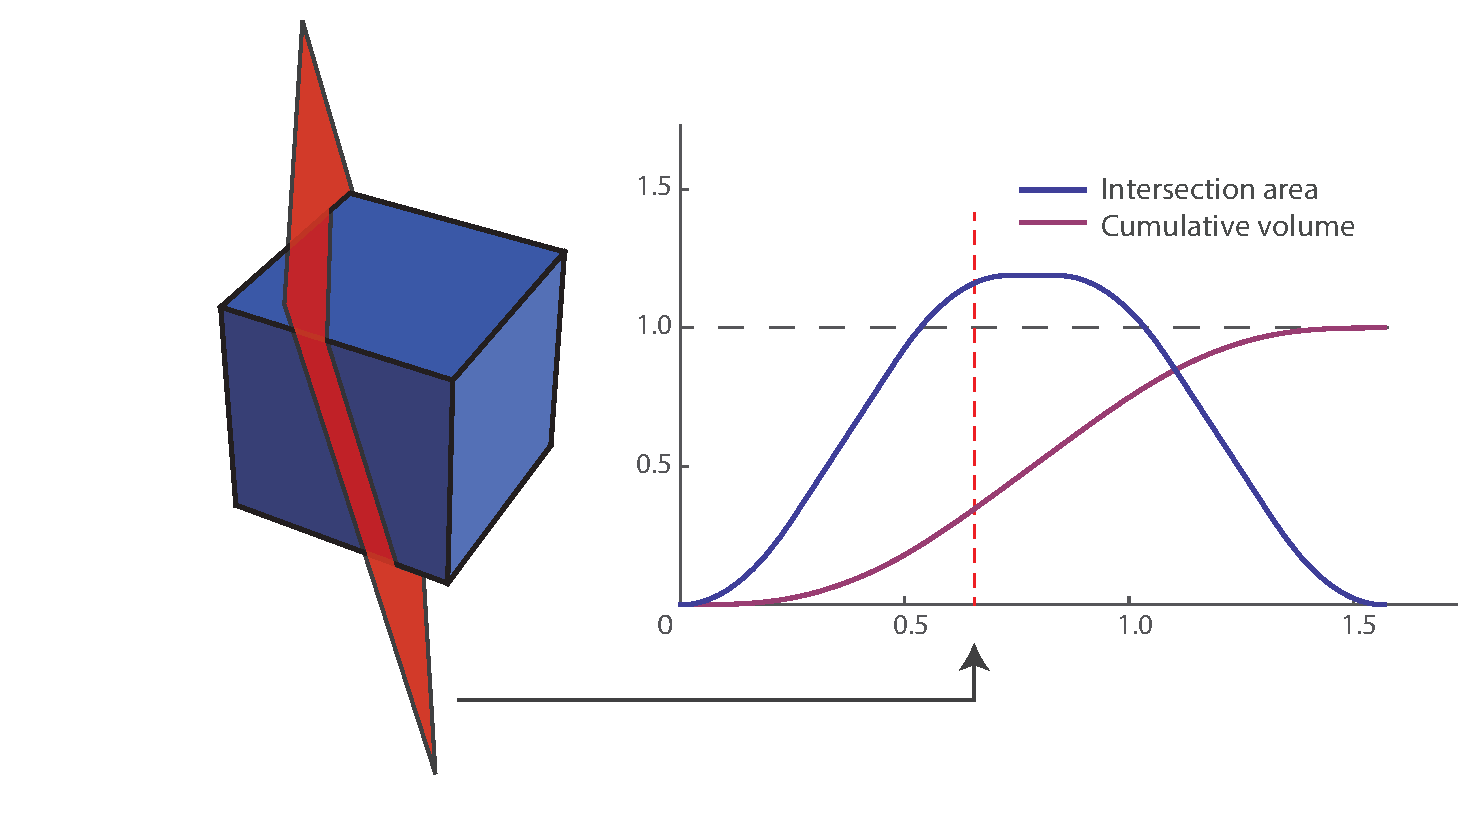
\includegraphics[width=1.\textwidth, clip=true]{./Chapters/03_GLM/./Images/Cube}
	\caption{The plane of arbitrary normal $\vec{n}$ (here $\vec{n}=(n_x, n_y, n_z)=(0.841, 0.480, 0.249)$) divides a unit voxel in two parts (red dashed line). As the plane moves in the direction its the normal, the area of intersection varies, as indicated by the blue curve. The volume within the voxel on the left side of the plane is indicated by the cumulative volume and represented by the purple curve.}
	\label{fig:cube}
\end{figure}
This procedure easily generalises to multiple layers being present in a single voxel, as it corresponds to an intersection with multiple planes. The volumes for the respective layers are hence given by the integral of the intersection area from one plane to the next. The gradient estimate is voxel specific rather than layer specific (i.e. planes are assumed to be parallel) and the same intersection function is used. \add{This is accurate as long as the voxel length is sufficiently smaller than the radius of curvature.}

\subsection{The laminar time course}
Once the layer volume distribution is constructed, it can be applied to MRI data. For all given voxels within a region of interest, the voxel signal values represent our measurement data $\mathbf{Y}$. The rows of the design matrix $\mathbf{X}$ give the fractions of the voxel volumes ascribed to the corresponding layer by the layer volume distribution. The layer estimates $\mathbf{\hat{B}}$ can be obtained by regression of $\mathbf{Y}$ against $\mathbf{X}$, given covariance matrix $\mathbf{\Omega}$. In order to obtain a laminar time course from an ROI in fMRI time series, the regression can be performed sequentially for that ROI. Note that the unmixing matrix is independent of the temporal signal, so the regressor calculation needs only to be performed once.

% % % %
\subsection{Similarity to existing methods} 
Hitherto, two main methods of extracting laminar time courses have been used. In the first one, the cortical surface is represented by two triangular meshes, the white matter surface and the pial surface. A laminar profile is then obtained by drawing lines from points (vertices) on one surface to the other. The volume projected onto these lines gives a cortical profile. In computing this projection, the volume has to be sampled by means of some interpolation method. This approach has been used in a number of implementations  \cite{Koopmans2011,Polimeni2010,DeMartino2013}. The second method is a classification of each voxel to be in a given layer based on the single most likely layer per voxel. The signal is subsequently averaged over the region of interest \cite{Siero2011,Olman2012,Maass2014}. Interestingly, all methods can be seen in the light of the same mathematical framework. 

% interpolation
Interpolating a volume at different cortical depths across a part of the cortex effectively creates a weighting for all voxels with respect to the layers. 
The weighting in this procedure is based on a limited set of vertices that form the mesh\remove{a weighting matrix}. While it is not guaranteed that all voxels in the region of interest are equally represented, one could likely assume that in the limit of an infinite number of lines the result would be similar to our laminar design matrix $\mathbf{X}$. The way in which the average is taken for all lines is then equivalent to a multiplication with the data, normalised with respect to the number of voxels:
\begin{equation}
\hat{\mathbf{B}}_{interpolation}= \mathbf{X^T} \cdot \mathbf{Y} / N.
\end{equation}
Here $\hat{\mathbf{B}}$, $\mathbf{X}$, and $\mathbf{Y}$ are respectively the estimated layer signals, the weighting matrix, and the voxel signals and have the same dimensions as in Eq.\ref{eq:glm}. $N$ is the number of voxels. We argue that such multiplication with our constructed design matrix is the best-case scenario of performance of the interpolation method.

% classification
Classification of voxels is a more direct attempt to obtain a layer volume distribution, with the property that all entries are binary, with exactly a single 1 in each row. Hence, by definition, the columns are orthogonal, and the average of the multiplication of an orthogonal design and the data is identical to regression of the data onto the same design. Therefore, classification can be viewed as a form of regression, but with a simplified design matrix. 

In the limit of infinite resolution, each voxel would fall into exactly one layer and it can readily be seen that all methods would be rendered equivalent. A similar scenario presents itself when the cortex is exactly aligned with the layering and each \change{layer}{voxel} falls into precisely one \change{voxel}{layer}. \change{In order to adequately compare all methods and reduce any bias induced by the variety of existing implementations, we here use the identical weighting matrices in the manner as described above.}{The aforementioned methods have been implemented in a variety of ways. Hence, the benefit of their descriptions in a consistent framework allows for easy comparison throughout the rest of this paper.}
\remove{
%%Add something here to give explicit plan of paper. 
To ascertain the behaviour of all methods, we first test the principles of the method on a simulated cortex of which we know that it behaves according to the equivolume principle. An OLS estimation is used, as there is no (un)correlated noise added to the system. In order to get a more detailed understanding of the behaviour of the method, we used high resolution (post mortem) data. The resolution and the anatomical detail allowed us to get a high number of layers and to assess a longer cortical profile. As the method is likely to be used on human in vivo data, we subsequently assessed anatomical profiles for 11 subjects. We give a detailed account of the influence of the extracted number of layers and we investigate the performance of different FWHMs that can be used for a GLS estimation.}